\documentclass{article}

\usepackage{graphicx} % Required for inserting images
\usepackage[
  autocite    = superscript,
  sortcites   = true,
  sorting     = none,
  style       = numeric,
  minbibnames = 3,
  ]{biblatex}

\title{\vspace{-2.5cm}Introduction of Photoconductivity}

\author{Jiakang Xu}
\date{December 2024}

\addbibresource{master_bib.bib}
\begin{document}

\maketitle



\section{Background pf photoconductivity}
In 1873 English electrical engineer Willoughby SmithOffsite Link discovered that the electrical resistance of selenium varies dramatically with the amount of light falling on it, which is the photoconductivity of selenium, and this is the first discovery of photoconductivity\parencite{Smith73}.
\section{Theory of Photoconductivity}
%ELI5 PC

%reminder of semiconductors and imperfections' effects. frame with "recombination centers" and stuff
The phenomenon of photoconductivity (PC) is most clearly observed in semiconductors, so we will first review some basic concepts of semiconductor physics\parencite{boer23}. The outermost electrons of atoms or molecules of a solid are found in energy "bands" composed of extremely densely distributed (but still discrete) energy levels. A material is a semiconductor if the outermost levels are close but do not quite overlap. When an electron is excited from the localized valence band, it becomes a freely moving charge carrier in the relatively nearby conduction band and leaves a positive "hole" in its previous place. The density of carriers determines the conductivity, and there is a temperature-dependent balance between thermal excitation and recombination (the process of an electron returning to the valence band), meaning semiconductors tend to conduct better the hotter they are (until it is so hot that thermal motion impedes electron drift).

Some semiconductors are doped with impurities, which may alter the normally equal balance between electrons and holes. Impurities may also act to provide intermediate energy levels between the valence and conduction bands. 

%basic PC: generation+recombo rates, steady states, dark vs photocurrent
Qualitatively, incident light can provide the energy required for electrons to jump to the conduction band, increasing conductivity from the dark conductivity(the conductivity with no light present). These electrons can be from the valence band in band-to-band absorption (intrinsic PC), or from an intermediate localized state from an impurity (extrinsic PC). When the light level is changed, the carrier generation vs. recombination balance is is shifted, changing the density of carriers in the steady state. This, depending on the substance, can take times of tens of milliseconds (sensitized photoconductors) to picoseconds (insensitized or normal photoconductors).

%intrinsic PC: basic explanation, some eqns.
For intrinsic PC, a photon is absorbed in the valence band and an electron is raised directly to the conduction band. This process creates equal numbers of electrons and holes, and is the main cause of photoconductivity in pure semiconductors. For our samples, vanadium oxide (VO$_{2}$), we expect only intrinsic PC unless there are significant unintended impurities, so we emphasize it here.

%MORE INTRINSIC THEORY.
When the light level is changed in an intrinsic photoconductor, the generation and recombination rates shift and take from picoseconds to tens of nanoseconds to reach a new equilibrium, since intrinsic PC is insensitized. This means we can ignore transient conductivity. Consider an intrinsic photoconductor with dark conductivity $\sigma_0$. The conductivity is proportional to $\mu_nn+\mu_pp$, where n and p are carrier densities of electrons and holes, and $\mu_n$ and $\mu_p$ are their mobilities. Defining $b=\mu_n/\mu_p$, the fractional increase in conductivity due to incident light $\Delta \sigma/\sigma_0$ can be written:

\begin{equation}
    \frac{\Delta \sigma}{\sigma_0} = \frac{\sigma_f-\sigma_0}{\sigma_0} = \frac{b\Delta n+\Delta p}{bn_0+p_0}
\end{equation}

Since $\Delta p = \Delta n$ in intrinsic PC and $p=n$ for pure samples, we can write:

\begin{equation}
    \frac{\Delta \sigma}{\sigma_0} \approx \frac{\Delta n}{n_0}
\end{equation}

In terms of resistances, this can be rewritten:

\begin{equation}
    \frac{R_0}{R_f}-1\approx\frac{\Delta n}{n}
\end{equation}

which allows us to measure the fractional change due to light of charge carriers and conductivity from resistance measurements, without knowing the shape of our samples. Knowing the shape, one can measure the carrier density directly. Note that the light is in general unevenly incident along the surface of the material, so the intrinsic values given here are actually averages.

%extrinsic PC: slow(traps)+fast rec. centers, photoionization cross sections
There are multiple kinds of extrinsic PC, but all of them involve local energy levels between the valence and conduction bands. For example, impurities may act as "traps" which sequester electrons and reduce photoconductivity, or they may act as reservoirs from which more electrons may be emitted, increasing photoconductivity. Some impurities Coulomb-attract electrons away from the conduction band, or effectively keep them in. Effects can also change depending on whether the impurity makes the material n-type or p-type, and extrinsic photoconductivity need not produce equal numbers of electrons and holes.

%quenching and persistent PC
Photoconductivity can be reduced in sensitized photoconductors by the introduction of more light of a different wavelength which interferes with slow recombination centers, effectively converting them into fast recombination centers. This can also be done by increasing the temperature and the electric field. Sometimes PC can last for days or months after the light is introduced, which is caused by a combination of very slow recombination centers and the requirement for current continuity. This is called persistent PC. Photoconductivity has a number of related effects, including the photovoltaic effect, photothermoelectricity, and the photo-Hall effect.

\section{4-terminal measurements}
The 4-terminal resistance measurements are one of the most common methods for a lock-in amplifier, as shown in figure~\ref{fig:4tm}
They have the advantage over simpler methods with two terminals that the 4-terminal resistance measurements removes the effects of contact resistance, as shown in figure~\ref{fig:2tmc} and \ref{fig:4tmc}\parencite{Neves24}. The Versalab uses 4-terminal measurement to obtain the more accurate resistance measurement values.
\begin{figure}[htbp]
    \centering
    \begin{minipage}[t]{0.3\textwidth}
        \centering
        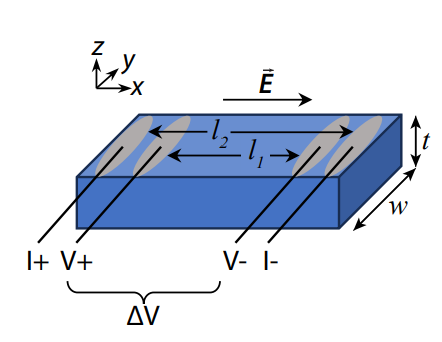
\includegraphics[width=\textwidth]{4tm.png}
        \caption{The 4-terminal measurement}
        \label{fig:4tm}
    \end{minipage}
    \hfill
    \begin{minipage}[t]{0.3\textwidth}
        \centering
        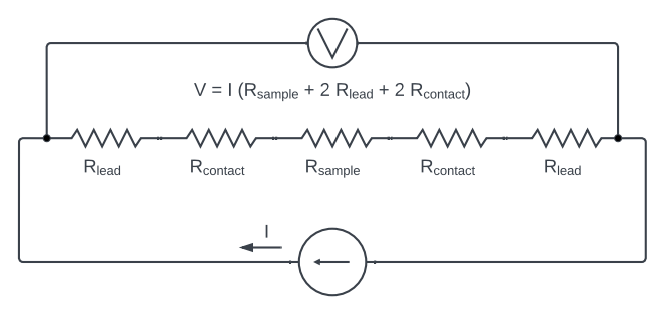
\includegraphics[width=\textwidth]{2tmc.png}
        \caption{The 2-terminal measurement circuit}
        \label{fig:2tmc}
    \end{minipage}
    \hfill
    \begin{minipage}[t]{0.3\textwidth}
        \centering
        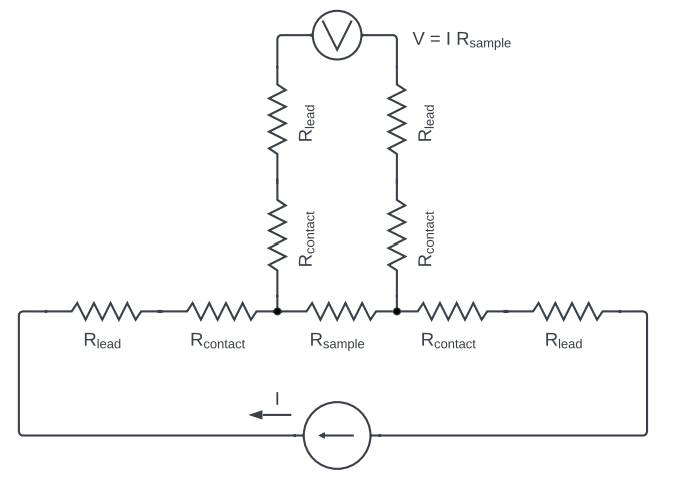
\includegraphics[width=\textwidth]{4tmc.png}
        \caption{The 4-terminal measurement circuit}
        \label{fig:4tmc}
    \end{minipage}
\end{figure}
\section{Vanadium(IV) oxide}
Vanadium(IV) oxide is an inorganic compound with the formula VO$_{2}$. It is a semiconductor at room temperature. However, the phase transition occurs around 340K, and VO$_{2}$ transfers from the monoclinic phase, which is semiconducting, to the rutile phase, which is metallic\parencite{Good71}, as the atoms in each pair separate, breaking the localized V-V bonds and releasing the bonding electrons,leading to a sharp increase in electrical conductivity\parencite{Green84}. The temperature of phase transition could be different in heating or cooling; the range of temperature in heating is 335-350K, while in cooling it is 340-325K\parencite{Morin59}. The optical band gap of VO2 in the semiconducting phase is about 0.7 eV\parencite{Shin90}.









\printbibliography

\end{document}
